%18/09 - Patricia Álvarez
\chapter{Ejercicios tipo examen}
\section{Ejercicio 1: Construir un árbol a partir de un alineamiento.}
Dado el siguiente alineamiento, construye un árbol filogenético. 
\begin{table}[h]
\centering
\begin{tabular}{l | l l l l }
\hline
& 1 & 2 & 3 & 4 \\
\hline
A & a & a & a & b\\
B & a & a & a & b \\
C & b & a & a & b \\
D & b & b & a & a \\
E & b & b & a & a \\
F & b & b & b & b
\end{tabular}
\end{table}

Hay varias formas de empezar. Una de ellas sería por aquellos que son iguales. Los taxones A y B son iguales, al igual que D y E. Por tanto, sabemos que esos taxones van juntos. Después, se busca el taxón más similar. En este caso, el taxón C es el siguiente más similar a los taxones A y B. Por último, el taxón F es el más diferente, siendo por tanto el outgroup. En resumen, el árbol quedaría así:

\begin{figure}[htbp]
\centering
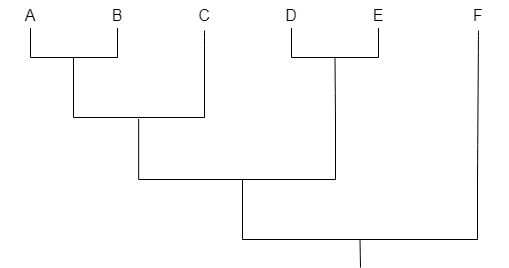
\includegraphics[width=0.7\linewidth]{figs/phylotree1.drawio.png}
\end{figure}

\section{Ejercicio 2: Construir la matriz de caracteres desde un árbol.}
Dado el siguiente árbol filogenético con las distintas mutaciones, construye una matriz de alineamiento.
\begin{figure}[htbp]
\centering
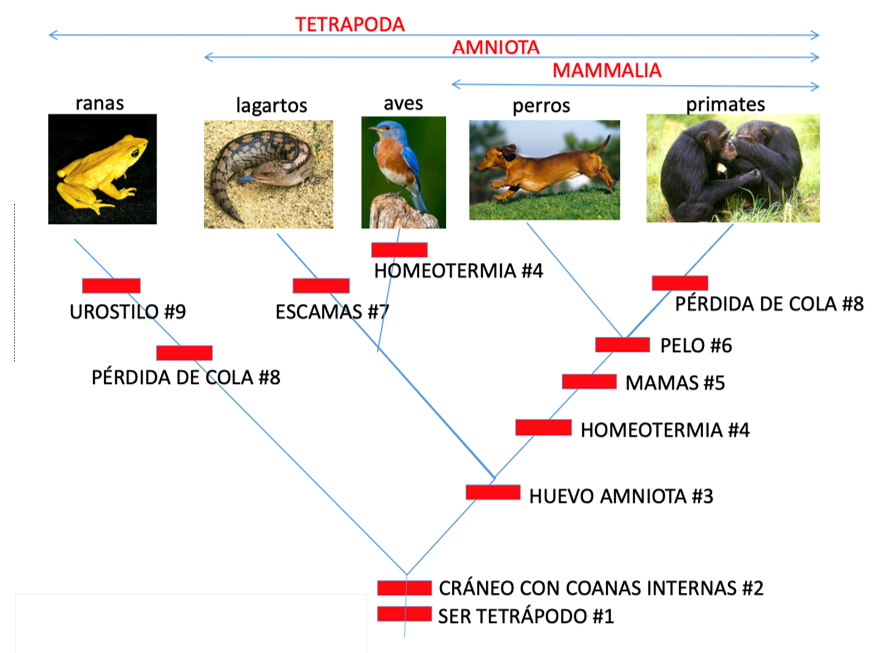
\includegraphics[width=0.7\linewidth]{figs/ejercicio-2.png}
\end{figure}

\begin{table}[htbp]
\centering
\begin{tabular}{l | l l l l l l l l l }
\hline
& 1 & 2 & 3 & 4 & 5 & 6 & 7 & 8 & 9 \\
\hline
Ranas & a & a & b & b & b & b & b & a & a\\
Lagartos & a & a & a & b & b & b & a & b & a\\
Aves & a & a & a & a & b & b & b & b & b\\
Perros & a & a & a & a & a & a & b & b & b\\
Primates & a & a & a & a & a & a & b & a & b
\end{tabular}
\caption{Matriz de alineamiento. La a indica presencia, la b indica ausencia}
\end{table}

\section{Identificación de caracteres}
En relación con el árbol filogenético del ejercicio 2, explica los caracteres en relación con todos los integrantes del árbol.

Los caracteres 1 y 2 son plesiomorfías al ser ancestrales. El carácter 3 es una sinapomorfía (sería una simplesiomorfía para los amniotas, pero como nos piden relacionarlo con todos los taxones, es una sinapomorfía del árbol). El carácter 9 es una autapomorfía de las ranas, y el 7 de los lagartos. El carácter 8 es otra autapomorfía con convergencia entre ranas y primates, generando así un grupo polifilético (el ancestro común más cercano no tiene el carácter). 

El grupo hermano de los amniotas son las ranas. Así, el grupo hermano de los mamíferos son lagartos y aves; no son los amniotas porque los mamíferos están englobados en los amniotas.  